\recipe[]{Negroni \& Americano}
\serves{1}%<----Numero di porzioni
\preptime{5 minuti}%<---Tempo di preparazione
\cooktime[]{-}%<-----Tempo di cottura
\autore{Max}
\begin{ingreds}
\ingredients[Negroni]
	50ml Gin \index{gin}
	50ml Vermouth rosso \index{vermouth}
	50ml Bitter \index{bitter}
	1 fetta d'arancia \index{arancia}
	Scorza d'arancia
	2 gocce di angostura (opzionali) \index{angostura}

\columnbreak

\ingredients[Americano]
	50ml Acqua tonica
	50ml Vermouth rosso
	50ml Bitter
	1 fetta d'arancia
	Scorza d'arancia
	2 gocce di angostura (opzionali)

\end{ingreds}

\begin{method}
Assembla il cocktail direttamente in un bicchiere old fashioned. Metti il giaccio, versa tutti gli ingredienti e mescola leggermente. Per l'Americano aggiungi l'acqua tonica solo alla fine.

Inserisci nel bicchiere una fetta d'arancia (indispensabile) e spruzza un po' di scorza di arancia sul bicchiere per profumarlo.

La lista degli ingredienti comprende solo i cocktails Americano e Negroni, tuttavia seguendo lo schema della figura \ref{negroni:schema} è facile produrre le altre varianti, ricordando che: Il bicchiere è sempre old fashioned, gli ingredienti vanno sempre divisi in partii uguali, la tonica va aggiunta sempre per ultima.
\end{method}

%\subsection*{Note}

% Figura
\begin{figure}[!h]
\centering
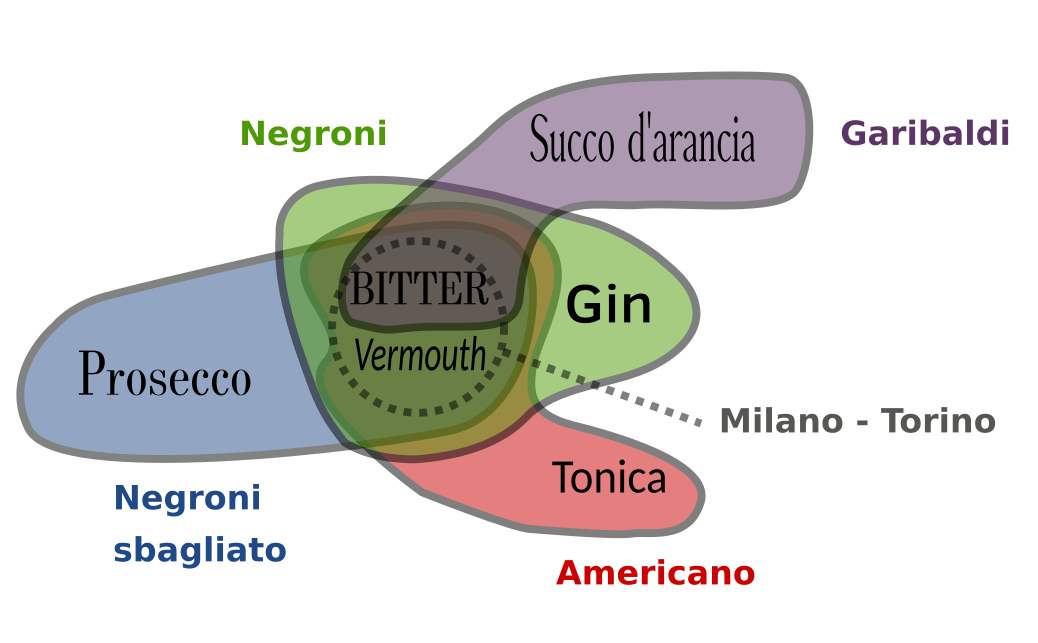
\includegraphics[]{img/negroni.png}
\caption{Il Negroni e i suoi derivati.}
\label{negroni:schema}
\end{figure}



